% Chapter Template

\chapter{Working Environment} % Main chapter title

\label{Chapter2} % Change X to a consecutive number; for referencing this chapter elsewhere, use \ref{ChapterX}

\lhead{Chapter 2. \emph{Working Environment}} % Change X to a consecutive number; this is for the header on each page - perhaps a shortened title

%----------------------------------------------------------------------------------------
%	SECTION 1
%----------------------------------------------------------------------------------------

%http://www.cisco.com/web/FR/documents/pdfs/livres_blancs/mobilite_sans_fil/Protocole_LWAPP.pdf

\section{UCL's Wireless Infrastructure}

On its Louvain-la-Neuve's campus area, the Catholic University of Louvain offers five different networks, each with a different \texttt{SSID}, that are reserved to certain parts of users according to their category. These available networks are the following:
\begin{itemize}
	\item[-] \texttt{student.UCLouvain}: Available for all the students enrolled at the Catholic University of Louvain.
	\item[-] \texttt{UCLouvain}: Reserved for the university's staff
	\item[-] \texttt{UCLouvain-prive}: Limited access to check the UCL's wireless configuration page or to download required programs for Windows XP and Windows Vista.
	\item[-] \texttt{visiteurs.UCLouvain}: Accessible for guests invited by the university.
	\item[-] \texttt{eduroam}: International education roaming access.
\end{itemize}

Network security is an important issue and an everyday struggle at the university and several measures are regularly taken by the SGSI team in order to keep the integrity and the consistency of the UCL's network preserved. As an example, Microsoft has decided on the 8th of April 2014 to end the Windows XP's support and updates leaving all the remaining laptops running this operating system unprotected to possible external threats \cite{windows}. The problem with that Microsoft's decision is that those outdated computers might become more vulnerable to security risks and malwares/viruses. It could turn into a real problem for the university's network because if a contaminated host is able to connect to the network it can cause serious damages to the overall infrastructure. In order to counter this possible problem, the SGSI team plan to block the wireless access using, for example, snorting programs, to any device that still runs on Windows XP.

The main way of protecting the UCL's network infrastructure from exterior threats that has been installed and configured by the SGSI team is the use of the \texttt{IEEE 802.1X} standard providing an authentication mechanism for all the devices that want to connect to one of the UCL's wireless networks. This architecture uses an authentication with user ID and password. Basically, every student, professor, researcher or staff members needs a \textit{username} and a \textit{password} in order to be able to establish a connection with one of the networks and get access to the Internet inside the UCL's campus. The username is composed of two parts, on one side the login the user has received from the university's administrative system when he enrolled himself, and on the other side the realm (\texttt{@wifi.uclouvain.be}). Along with that username, the user also needs a password. This password is the same as the password he uses to connect to his personal virtual office on the university's web site. Without those credentials it is impossible for him get an Internet connection within the university's campus.

This kind of authentication mechanism is only possible if the infrastructure has several key entities that are going to handle all this security authentication process. Those entities are an \textit{Authentication Server} and an \textit{Authenticator}.

Typically an Authentication Server is a host that supports the \texttt{RADIUS} and  \texttt{EAP} protocols. In the case of the UCL's infrastructure the Authenticator Server is also composed of several database servers, placed behind a load balancer, that support the \texttt{LDAP}\footnote{Lightweight Directory Access Protocol} protocol and where all the information about the students, professors, researchers and staff members of the UCL as well as a lot of other data are stored. Among those stored data, we find all the users' credentials.

The Authenticator is composed of the access point that handles the connection request from the user and the Cisco controller that handles all the authentication process. This authenticator is the real security guard for the network since the client is not allowed to access to the protected side of the network until it's identity has been checked and validated. Let's keep in mind that these controller and access point do not play a role in the real world of the authentication itself. They are called the \textit{Authenticator} because that is where the client asks for authentication but they do not authenticate the client. The device that authenticate the client is the \textit{Authentication Server}.

The following figure represents the architecture with the different components that handles the \texttt{802.1X} authentication process at the UCL. 

\begin{figure}[H]
	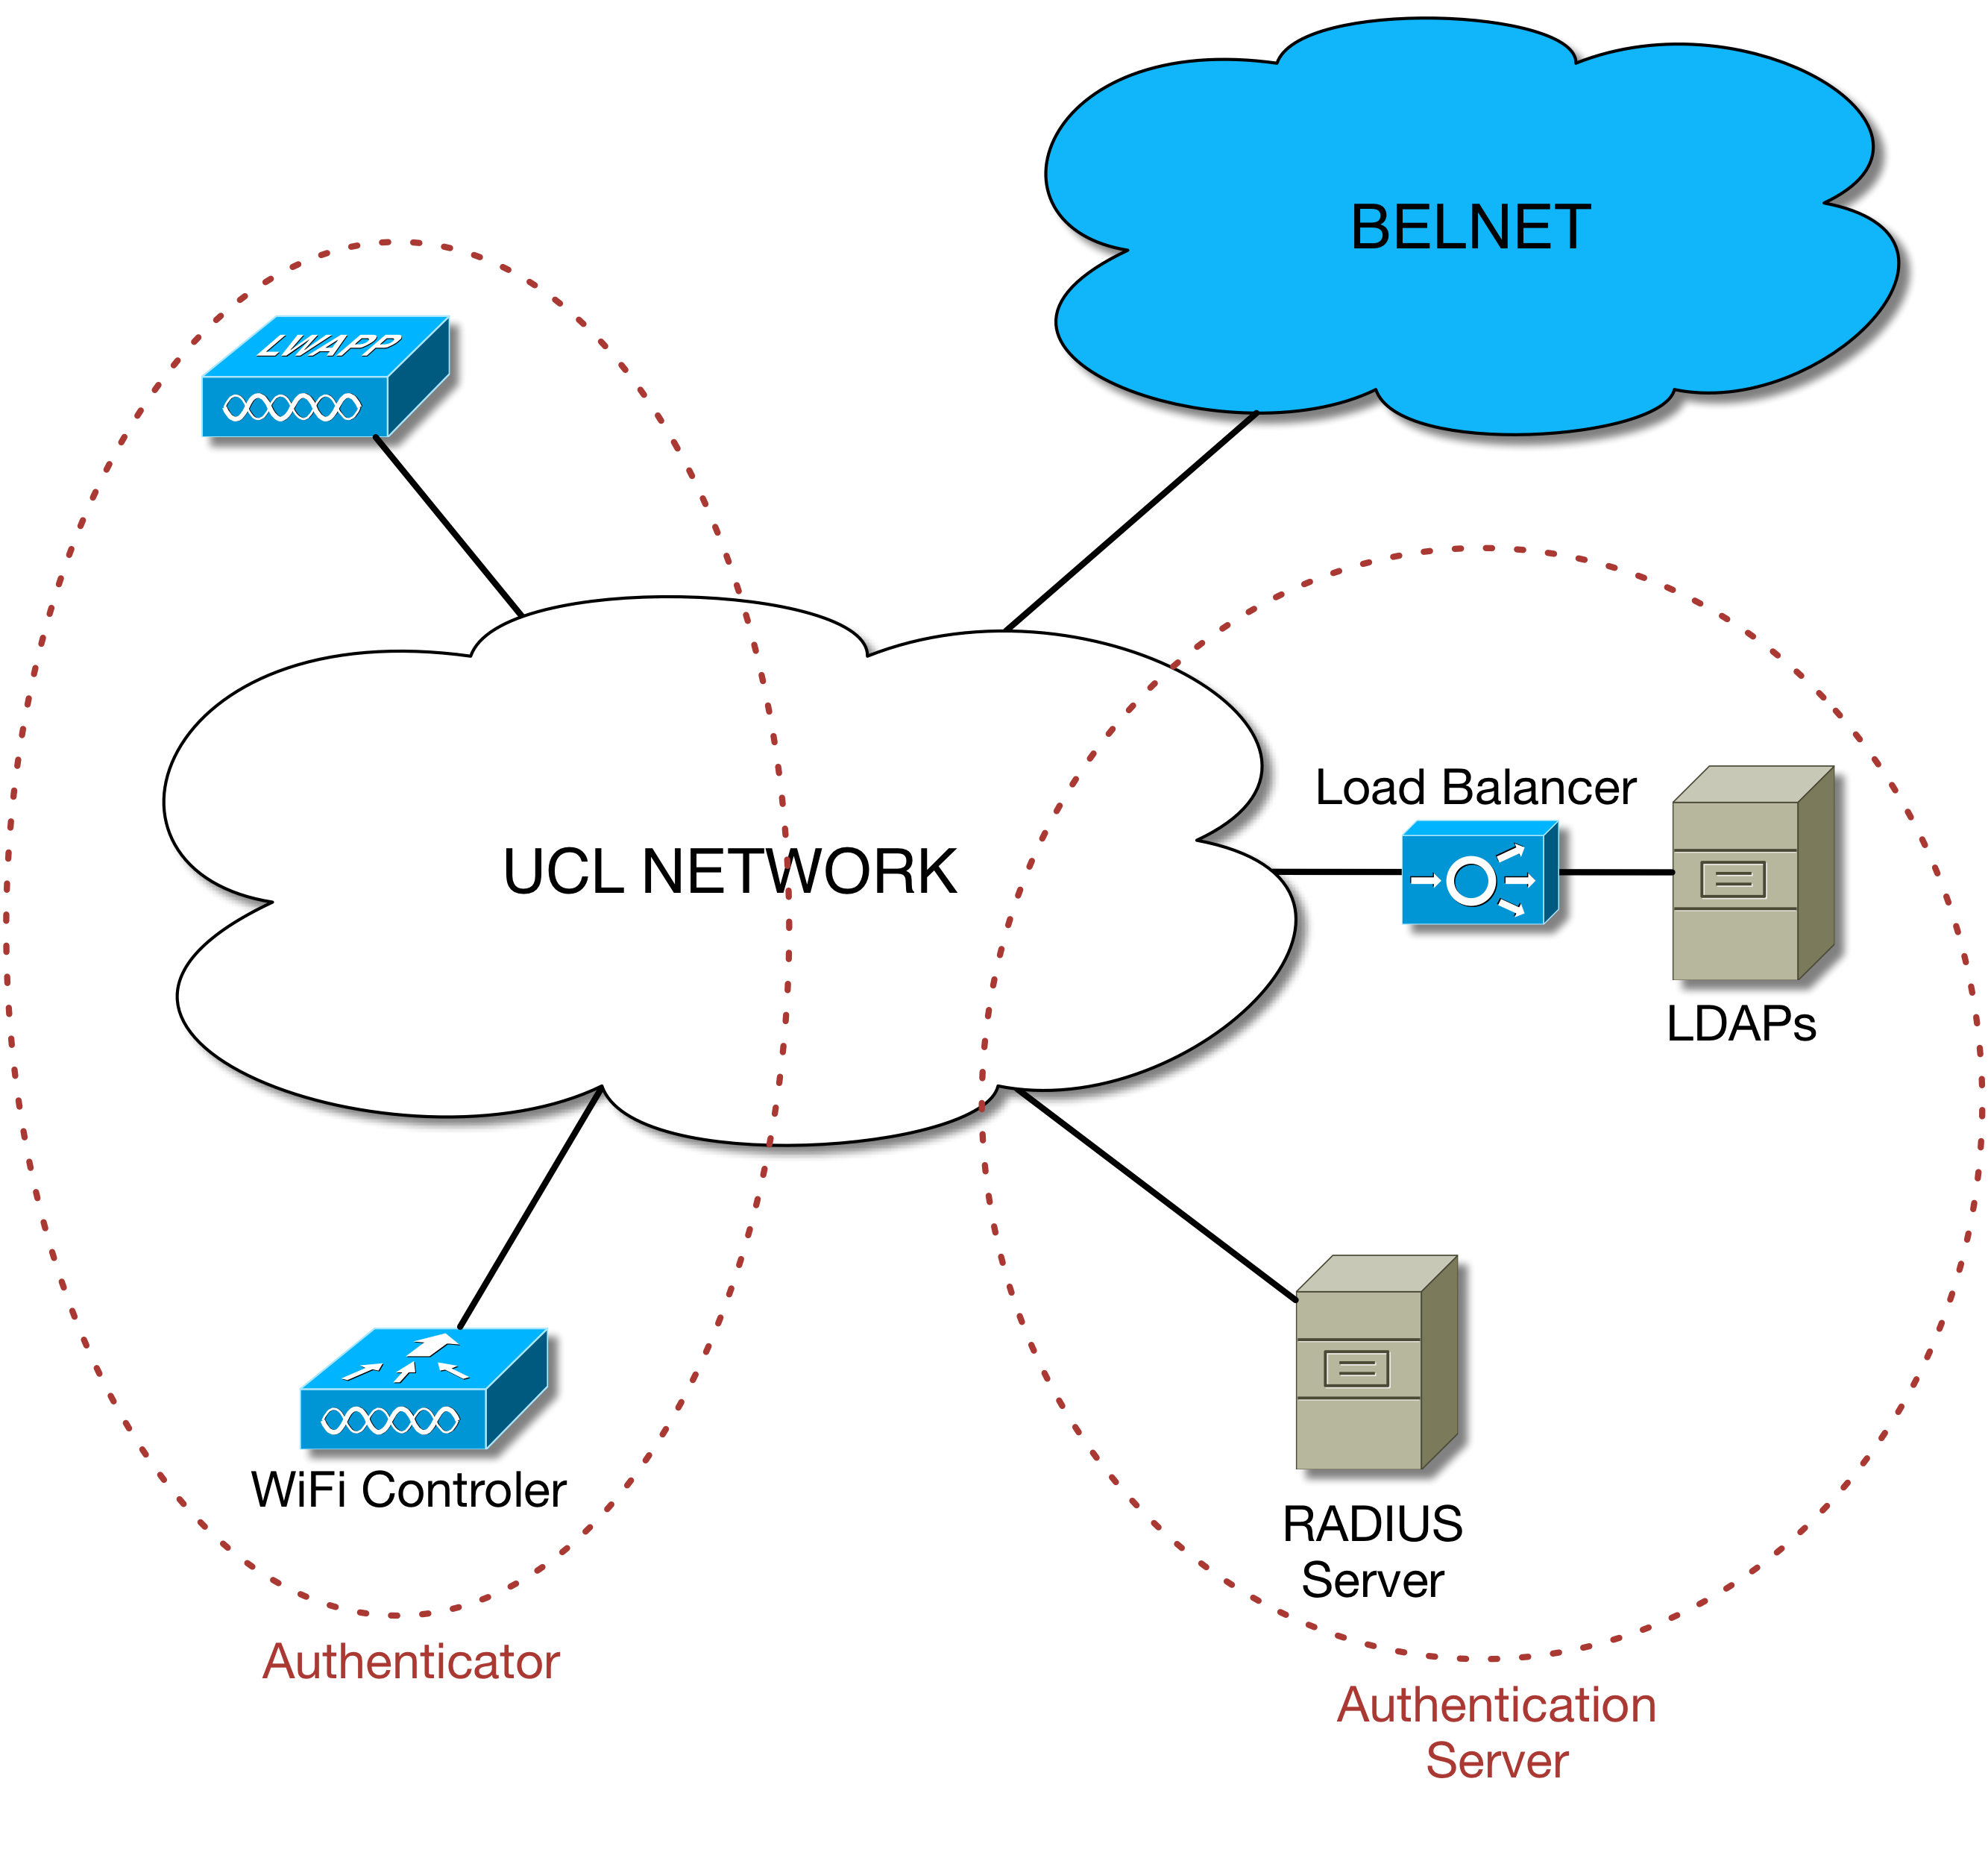
\includegraphics[width=1\linewidth]{Pictures/chapter2/802-archi.png}
	\caption{\texttt{802.1X} architecture and components at the UCL}
\end{figure}



\section{Network Components and Protocols}
In this section, we give more information and details about all the protocols and components used throughout this thesis.

\subsection{EAP}
The \textit{Extensible Authentication Protocol} is an Internet Engineering Task Force (IETF) flexible authentication framework standard defined in the \texttt{RFC3748} \cite{rfc3748}. \texttt{EAP} was designed to work without the IP protocol and provides support only for the transport of authentication protocols. This protocol runs directly over data link layers such as \texttt{Point-to-Point Protocol} (PPP) or \texttt{IEEE 802}. It is used to select a specific authentication mechanism whenever the authenticator requests more information to the supplicant.

The particularity with \texttt{EAP} is that the authentication mechanism is negotiated by the peers (i.e. the supplicants) during the connection authentication phase with the authentication server. The peers negotiate the use of which \texttt{EAP} method to use during the authentication. Once the method has been agreed upon, an \texttt{EAP} conversation consisting of requests and responses messages exchanged between the peer and the authentication server starts.

The \texttt{EAP} architecture consists of three main elements:
\begin{itemize}
	\item \textbf{EAP peer}: The peer is the client that tries to access the protected network and that responds to the authenticator requests.
	\item \textbf{EAP authenticator}: It is the end of the link initiating an \texttt{EAP} authentication process. It is the access point or the network access server that requires \texttt{EAP} authentication in order to grant access to the network.
	\item \textbf{Authentication server}: The server that communicates with the \texttt{EAP} peer. It negotiate the \texttt{EAP} method to use and validates the peer's credentials allowing it to access the protected network or not.
\end{itemize}

Since \texttt{EAP} only defines message formats it has to be encapsulated inside a data link layer transport protocols. Between the peer and the authenticator, the \texttt{EAP} messages has to be encapsulated inside protocols such as \texttt{PPP}, \texttt{PEAP} or \texttt{IEEE 802.1X}. The encapsulation of \texttt{EAP} over \texttt{IEEE 802.1X} is called \texttt{EAPOL}\footnote{EAP over LANs}. Once the authenticator has received a \texttt{EAP} message from the peer, it has to forward it to the authentication server and it does that by encapsulating the message using that \texttt{RADIUS} protocol. Thanks to that, the \texttt{EAP} messages are exchanged between the peer and the authentication server smoothly. Since the information flows between those two entities, the authenticator does not need to support any of the \texttt{EAP} methods. It just has to forward the messages.

The following figure\footnote{http://technet.microsoft.com/en-us/library/bb457039.aspx} shows the \texttt{EAP} infrastructure and the information flow between the three components.

\begin{figure}[H]
	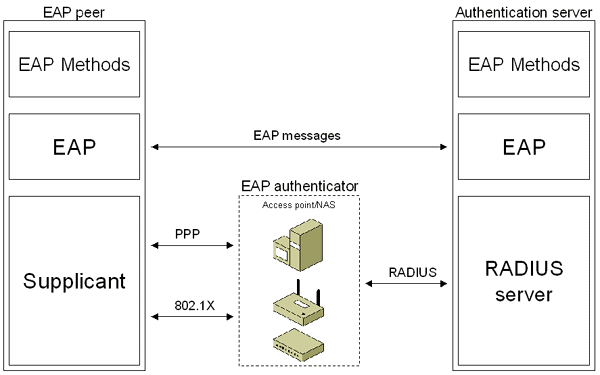
\includegraphics[width=1\linewidth]{Pictures/chapter2/eap.png}
	\caption{\texttt{EAP} infrastructure and information flow}
\end{figure}

The \texttt{EAP} method requirements for Wireless LANs is defined in the \texttt{RFC4017} \cite{rfc4017}. The methods used in today's wireless LANs includes \texttt{EAP-TLS}, \texttt{EAP-TTLS} and \texttt{PEAP}. As mentioned in the RFC, these methods support authentication credentials that include digital certificates, user-names and passwords, secure tokens, and SIM secrets.

\subsubsection{EAP-TLS}
Defined in \texttt{RFC5216} \cite{rfc5216}, the \texttt{EAP-TLS} authentication protocol includes support for certificate-based mutual authentication and key derivation, utilizing the protected cipher suite negotiation, mutual authentication and key management capabilities of the \texttt{TLS} protocol discussed in \texttt{RFC4346} \cite{rfc4346}. The security with this protocol is provided by the utilization of \texttt{X.509} certificates. Indeed, in the \texttt{TLS} negotiation, the server presents a certificate to the client, and if mutual authentication is requested, the peer also presents its certificate to the server.

\subsubsection{EAP-TTLS} 
This protocol, defined in the \texttt{RFC5281} \cite{rfc5281}, extends \texttt{TLS}. It uses \texttt{TLS} to establish a secure connection between the client and the server, through which additional information may be exchanged. The difference with \texttt{TTLS} is that one-way authentication in which only the server is authenticated to the client via its certificate is possible. Once the secure tunnel is established between them, the client can send its credentials (i.e. username and password).

\subsubsection{PEAP} 
The Protected Extensible Authentication Protocol is defined in the \texttt{IETF} draft \cite{peap-draft}. This protocol provides an encrypted and authenticated tunnel based on \texttt{TLS} that encapsulates \texttt{EAP} authentication mechanisms. \texttt{PEAP} works by chaining multiple \texttt{EAP} mechanisms. Basically it is composed of two parts. First, a \texttt{TLS} session is negotiated with the server authenticating to the client and optionally the client to the server. The negotiated key is used to encrypt the rest of the conversation. Second, within that \texttt{TLS} session, zero or more \texttt{EAP} methods are carried out.
The most common version of \texttt{PEAP} is \texttt{PEAP-MSCHAPv2}. This version uses the Microsoft Challenge Handshake Authentication Protocol version 2 (described in section \texttt{2.2.3.1}) for the inner authentication method.



\subsection{IEEE 802.1X}
%http://www.blackhat.com/presentations/win-usa-03/bh-win-03-riley-wireless/bh-win-03-riley.pdf
\texttt{802.1X} is a Port-based Network Access Control that is part of the \texttt{IEEE 802.1} group of networking protocols. Basically, it is a way of securing a network access and doing authentication over ports to devices wishing to attach to a \texttt{LAN} or a \texttt{WLAN}. It offers an effective framework for authenticating and controlling user traffic to a protected network.

The \texttt{802.1X} authentication process architecture involves three main components:
\begin{itemize}
	\item[-]\texttt{Supplicant}: The client device that wants to connect to the network.
	\item[-]\texttt{Authenticator}: A network device like an Ethernet switch or an access point that is between the supplicant and the authentication server. It purpose is to interact with the authentication server. It receives \texttt{EAP} messages, encapsulates them into \texttt{RADIUS} messages and forwards them to the authentication server.
	\item[-]\texttt{Authentication Server}: It is the key part of that authentication process. This server receives the authentication requests from the authenticator and interacts with it in order to receive more information or credentials from the supplicant. It is the only one that can grant access or not to the protected network.
\end{itemize} 

This protocol is called \textit{Port-based Network Access Control} because the ports of the authenticator (i.e. the access point) are configured in a certain way. Indeed, before being totally open, the ports only accept \texttt{EAP} messages. The design is that each port is divided into two different parts. One part is the \textit{controlled} part of the port and the other is the \textit{uncontrolled} part of the port. The main idea is that all the \texttt{EAP} messages go through this uncontrolled port and only when the supplicant is granted access to the network, it can go through the controlled one.

\texttt{802.1X} works either for \texttt{WLAN} or \texttt{LAN} authentication but the authentication flow is not exactly the same. In our thesis we focus on the \texttt{WLAN} authentication.

For \texttt{WLAN} authentication, the first thing the supplicant does is to associate with the access point using standard \texttt{802.11} communication. Once the association is made, the supplicant encapsulates its information and authentication requests inside \texttt{EAP} messages and sends them to the authenticator through the uncontrolled port. The authenticator encapsulates those messages into \texttt{RADIUS} packets and forwards them to the authentication server. Then, after having set up a secure and encrypted tunnel with the supplicant, the authentication server starts communicating with it (to receive its username and password for example). The server then queries its database and finally, if the user is known by the database, the server asks the authenticator to open completely the port so that the user can access freely the requested \texttt{VLAN}.

The following figure represents this authentication mechanism. First, the supplicant communicates with the authenticator (1). Then after the authenticator has forwarded the messages to the authentication server and after the secured tunnel between the supplicant and the server has been set up, those two components can start exchanging messages (2). Finally, if the authentication is a success, the supplicant has access to the protected network (3).

\begin{figure}[H]
	\begin{center}
	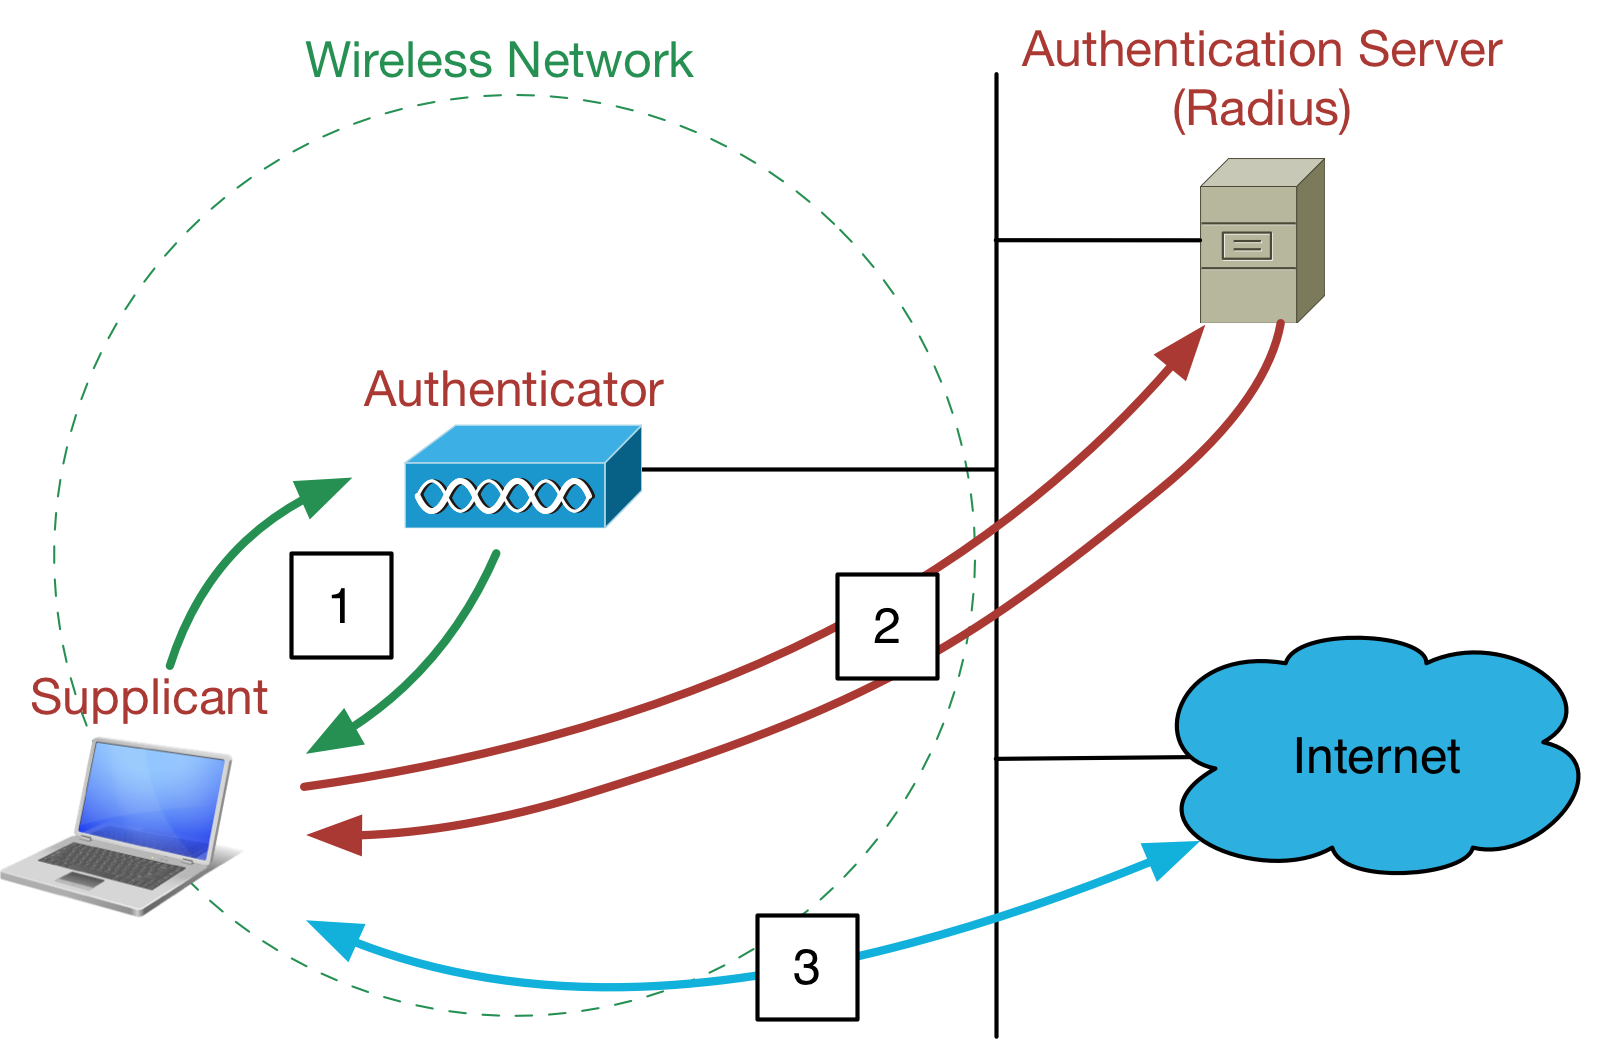
\includegraphics[width=.7\linewidth]{Pictures/chapter2/802.png}
	\caption{\texttt{802.1X} authentication mechanism for WLAN}
	\end{center}
\end{figure}


\subsection{RADIUS}
The Remote Authentication Dial In User Service is defined in \texttt{RFC2865} \cite{rfc2865} and \texttt{RFC2866} \cite{rfc2866}. This is a networking protocol that provides Authentication, Authorization and Accounting (\texttt{AAA}) management for users that connect and use a network service. \texttt{RADIUS} is a client/server protocol that uses \texttt{UDP} for the communications between the \texttt{NAS}\footnote{Network Access Server} and the \texttt{RADIUS} server. It uses port \texttt{1812} for authentication and authorization requests and port \texttt{1813} for accounting requests. The process of granting a supplicant the access to a protected network is divided in three steps.

\subsubsection{Authentication}
The supplicant sends a connection request to a \texttt{RADIUS} client, called the \texttt{NAS}, in order to get access to a particular network resource. The supplicant credentials (i.e. username and password) are also transmitted by the supplicant to the \texttt{RADIUS} client. Once the client has received the request and credentials, it sends a \texttt{RADIUS} \textit{Access-Request} message to the \texttt{RADIUS} server containing all the authentication information. The server checks if that information is correct by checking that it against a local database or by referring to external sources, such as \texttt{LDAP} servers, to verify the user's credentials. This checking process is done using authentication schemes such as \texttt{CHAP}, \texttt{MS-CHAP}, or \texttt{EAP}.
	\begin{itemize}
		\item [-] \texttt{CHAP}: The \textit{Challenge-Handshake Authentication Protocol}, defined in \texttt{RFC1994} \cite{rfc1994}, is an authentication scheme used by \texttt{PPP}\footnote{Point to Point Protocol} servers to periodically verify the identity of the user using a three-way handshake. The first step in the \texttt{CHAP} protocol is to establish a \texttt{LCP}\footnote{Link Control Protocol} link by the supplicant with the authenticator. Once the link is established, the authenticator sends a \textit{Challenge} message to the supplicant. The latter responds with a value calculated using a one-way hash function and a shared secret (such as the user's password) combined. The authenticator does the same computation with the same one-way hash function and checks the response received by the supplicant against its own result. If values matches, the authentication is acknowledged, otherwise the connection should be terminated. Finally, the authenticator sends a new challenge to the supplicant at random intervals and repeats the steps described before.

		\item [-] \texttt{MS-CHAP}: The main constraint encountered with the \texttt{CHAP} protocol is that the supplicant and the authenticator need to share a common secret (i.e. a password). The \texttt{MS-CHAP} has been developed by Microsoft in order to delete this constraint. Two versions of this protocol exist: \texttt{MS-CHAPv1}, defined in \texttt{RFC2433} \cite{rfc2433}, and \texttt{MS-CHAPv2}, defined in \texttt{RFC2759} \cite{rfc2759}. Version 2 is the one used inside the UCL's network authentication process since it offers stronger security for remote access connection. It features a two-way authentication verification of the identity of both sides of the connection. Also, separate cryptographic keys are used for data transmission and reception and each time the user connects with the same password, a different cryptographic key is used.

		\item [-] \texttt{EAP}: The \textit{Extensible Authentication Protocol} is detailed in section \text{2.2.1}.
	\end{itemize}

The server then returns one of the three \texttt{RADIUS} responses to the client:
	\begin{description}
		\item [Access-Challenge]: If the \texttt{RADIUS} server needs additional information from the supplicant, it sends this packet to the client requesting that information. The client responds with a new \textit{Access-Request} message. \textit{Access-Challenge} is also used in complex authentication process when a secure tunnel is established between the supplicant and the \texttt{RADIUS} server.

		\item [Access-Accept]: The server grants access to the supplicant.

		\item [Access-Reject]: The server denies access to the supplicant due to identification failure, unknown or inactive user.
	\end{description}

The following figure represents the message exchanges between a \texttt{NAS} and the \texttt{RADIUS} server. The server needs and asks for additional information in the authentication process and finally grant the access to the network.

\begin{figure}[H]
	\begin{center}
		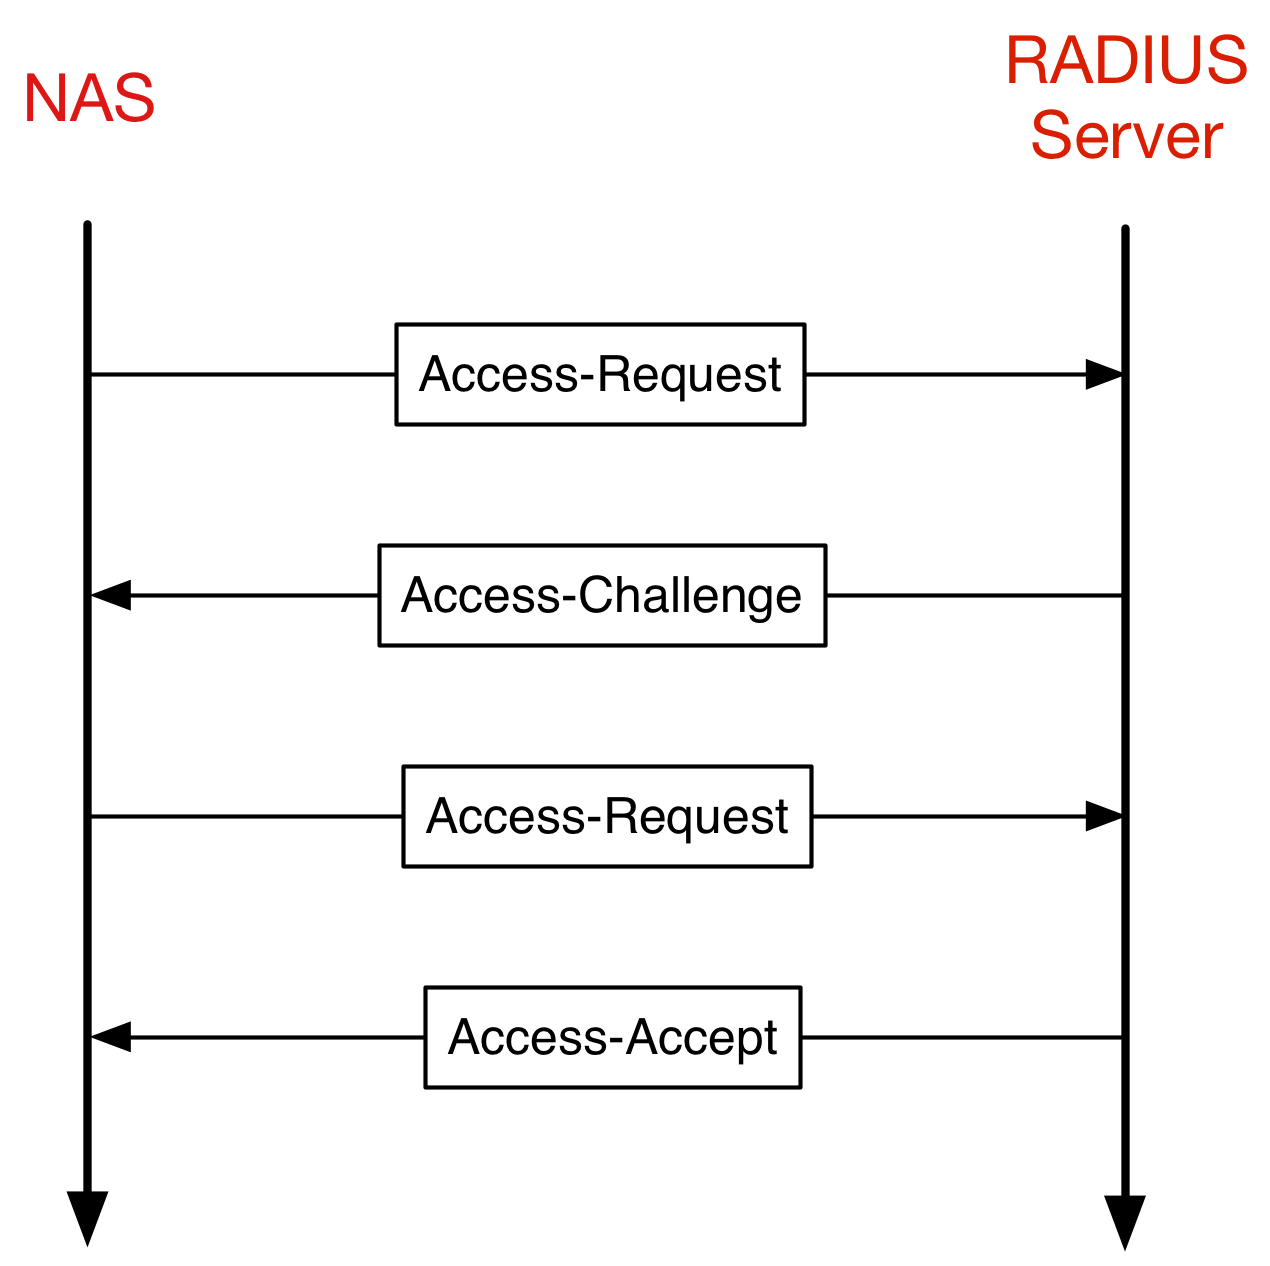
\includegraphics[width=.5\linewidth]{Pictures/chapter2/radius-authentication.png}
		\caption{\texttt{RADIUS} authentication process and message exchanges}
	\end{center}
\end{figure}
		
\subsubsection{Authorization}
Once \texttt{RADIUS} server has successfully authenticated the user, it can return configuration information to the client (i.e. authorization attributes), stipulating the terms of access to be granted, inside the \textit{Access-Accept} response. Different attributes may be included such as:
		\begin{itemize}
			\item [-] Specific IP address

			\item [-] Maximal length the user may remain connected

			\item [-] \texttt{VLAN} parameters

			\item [-] \texttt{QoS} parameters
		\end{itemize}
	The complete list of possible attributes can be found in \cite{rfc2865}.

\subsubsection{Accounting}
The accounting uses three types of packets, \textit{Accounting Start}, \textit{Interim Update} and \textit{Accounting Stop}. The first packet is transmitted by the \texttt{NAS} to the \texttt{RADIUS} server as soon as the user authentication has succeeded and that he has started to access the network. This packet contains several information about the user such as his username, his affected IP address, the date of connection, and so on. The last packet is sent when the user disconnects from the network. Upon reception of that \textit{Accounting Stop} packet, the sever can end the user's session and log all the information about that particular session. The \textit{Interim Update} packet is sent by the \texttt{NAS} to update the information of the current session. All these packets are encapsulated inside an \textit{Accounting-Request} \texttt{RADIUS} message. The server responds with a \textit{Accounting-Response} message. The purpose of the accounting is to keep a trace of everything that happens on the network and to keep data about all the users that have accessed it. Plus it is also used for statistical analysis and network monitoring.

	The following figure depicts the accounting messages flow between the \texttt{NAS} and the \texttt{RADIUS} server. On packet of each type is represented to get a better overview.

	\begin{figure}[H]
		\begin{center}
			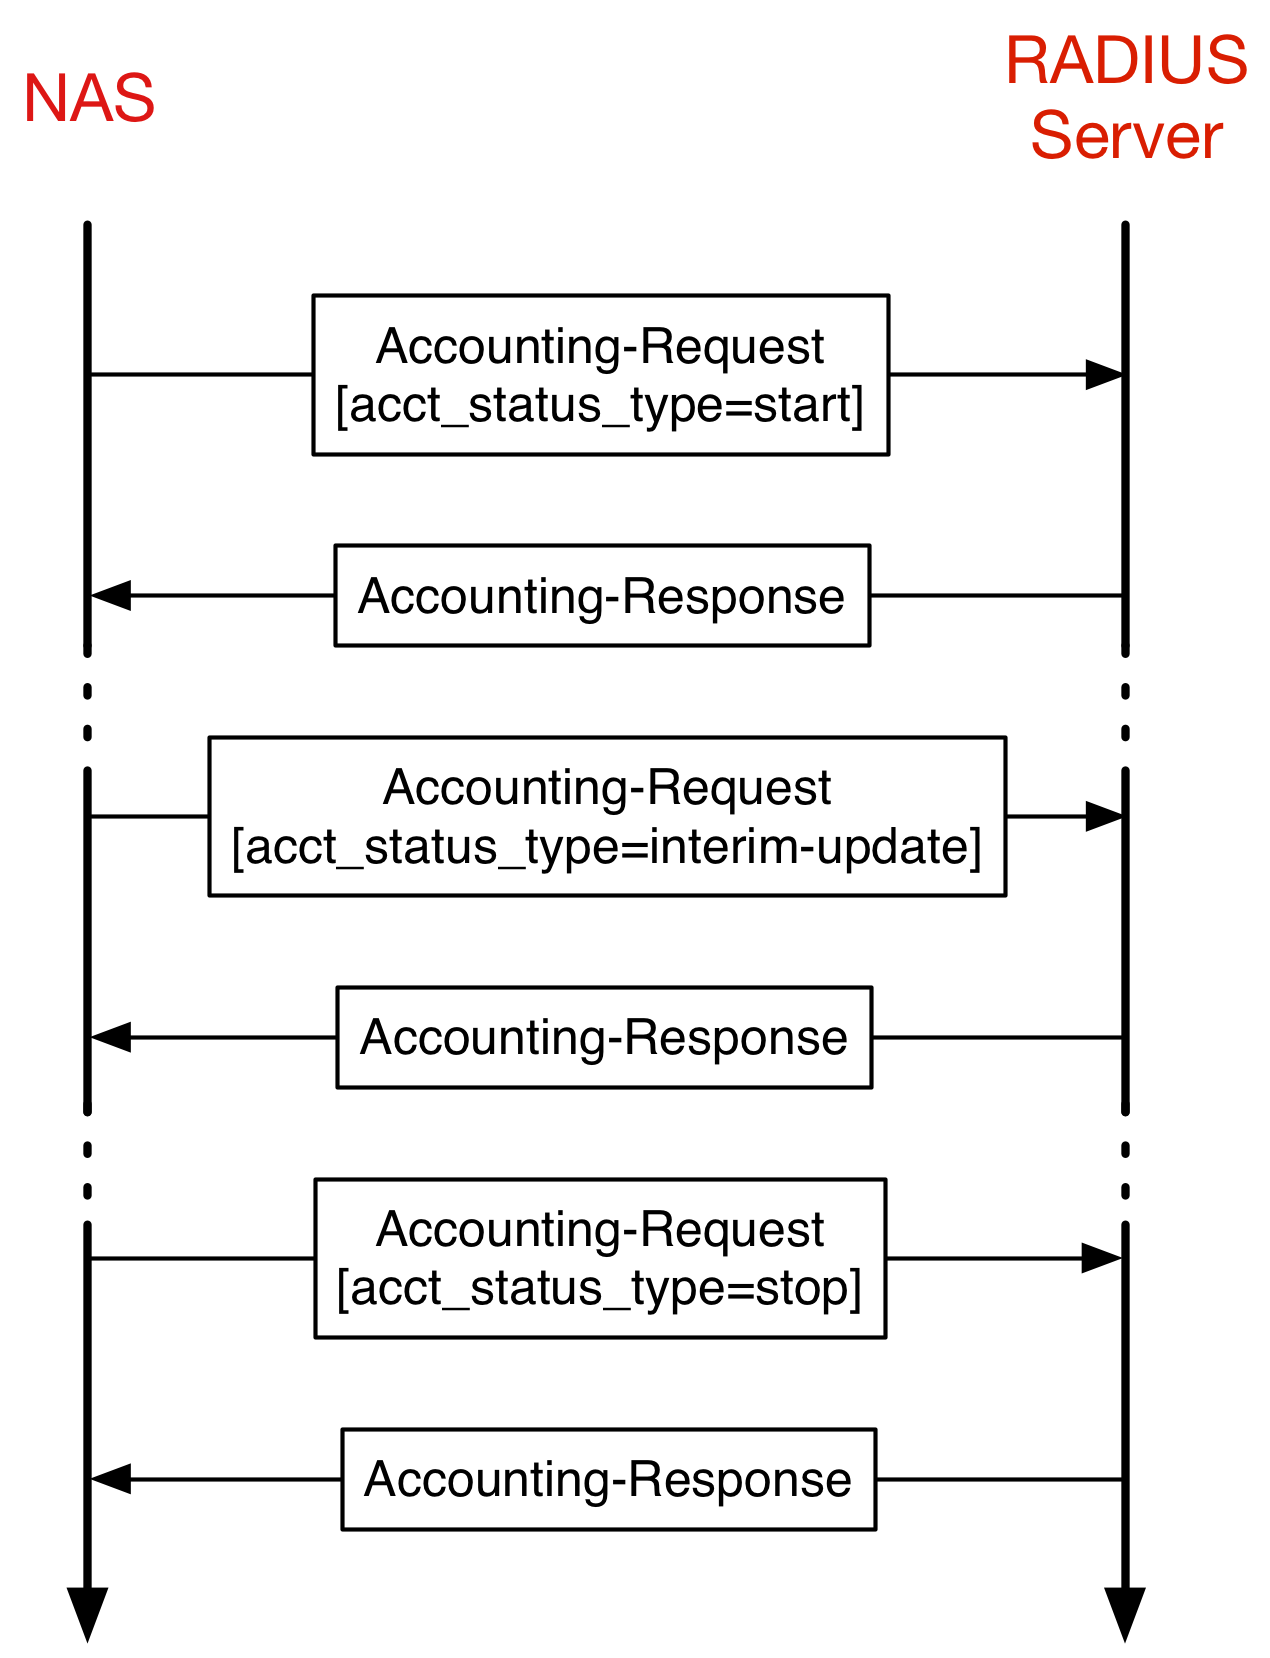
\includegraphics[width=.5\linewidth]{Pictures/chapter2/radius-accounting.png}
			\caption{\texttt{RADIUS} accounting messages flow}
		\end{center}
	\end{figure}


\subsection{WiSM2}
The Cisco Wireless Service Module 2 Controller (\texttt{WiSM2}) is, as described in \cite{wism2}, a highly scalable and flexible platform that enables system-wide services for mission-critical wireless networking in medium-sized to large enterprises and campus environments. This controller, designed to occupy one slot into a \texttt{Cisco Catalyst 6500 Series Switch}, supports up to 1,000 access points and 15,000 clients and is optimized for \texttt{802.11n} networks. It also contains two WLCs\footnote{Wireless Lan Controller}.


\subsection{SNMP}

The Simple Network Management Protocol is an application layer protocol that facilitates the exchange of management information between network devices \cite{snmp}. It is part of the \texttt{TCP/IP} protocol suite and it is mainly used by network administrators to get information about devices on the network and the network performances. These information help the administrators to resolve problems on the network or simply to manage any network device that is configured with \texttt{SNMP} agent software. A \texttt{SNMP} network has three main components:

\begin{description}
	\item [Network-Management System]: A \texttt{NMS} is the main component of an \texttt{SNMP}-managed network. It is the management entity that controls the managed devices. It uses the \texttt{SNMP} protocol and can interact with the managed devices to get information using special commands and messages.
	
	\item [Managed Devices]: It is a network device, i.e. a node, that contains an \texttt{SNMP} agent. They collect and store information to make them available for the network-management systems. Those devices can be routers, servers, switches, etc. They also run the \texttt{SNMP} protocols to be able to respond to the requests made by the \texttt{NMS}.
	
	\item [Agents]: An agent is the thinking part of a managed device. It is a software module that understands the management information and translates them into a \texttt{SNMP} compatible form.
\end{description}

\begin{figure}[H]
\centering
	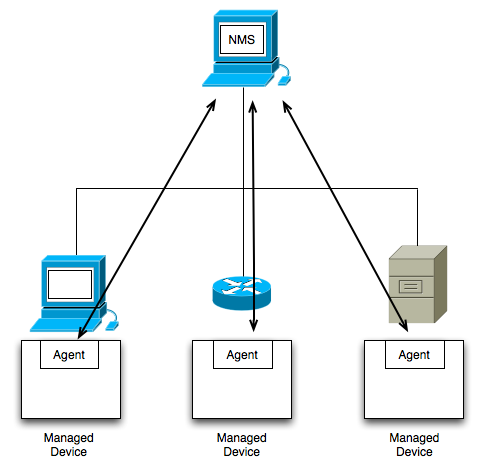
\includegraphics[width=.7\linewidth]{Pictures/chapter2/snmp.png}
	\caption{A typical \texttt{SNMP} managed network}
\end{figure}

All the network objects are described and organized hierarchically in a Management Information Base (\texttt{MIB}). There are \texttt{MIBs} for each set of related network entities that can be managed. These \texttt{MIBs} are accessed using a network-management protocol such as SNMP. There are two types of \texttt{MIBs}: \textit{scalar} and \textit{tabular}. Scalar objects define a single object instance while tabular objects define multiple related object instances grouped in \texttt{MIB} tables.Managed objects of a \texttt{MIB} hierarchy are identified by an Object Identifier (\texttt{OID}).



\section{WLAN authentication process}
Let's analyze the authentication process mechanism with a WLAN network.
As explained before, with the \texttt{IEEE 802.1X} standard, there are two key parts, the \textit{Authenticator} and the \textit{Authentication Server}. In the case of a WiFi authentication process, a third one can be added to this list and is called the \textit{Supplicant}. The supplicant is simply the wireless client that asks for an authentication in order to have access to the protected network. The authentication process works in several key steps and uses different protocols.

First of all, the supplicant who wants to access the network needs to make a special request to the authenticator. During that step the protocols that are used between the supplicant and the authenticator are a combination of \texttt{802.1X} and \texttt{EAP} protocol (\textit{Extensible Authentication Protocol}). Thanks to \texttt{802.1X} protocol, the authenticator can refuse any access to the network as long as the authentication server has not authenticated the client and accepted to open the access (i.e. open the port). The \texttt{EAP} defines a standard for the messages that are going to be exchanged between the supplicant and the authentication server. It is a  transport protocol for the authentication protocols. Those \texttt{EAP} messages are encapsulated over \texttt{IEEE 802} and this encapsulation is known as \texttt{EAPOL} (for \textit{"EAP over LAN"}. Technically we should say \texttt{EAPOW} for a wireless network but it is only to refer to an \texttt{EAPOL} message that is being sent using \texttt{802.11} wireless network transmission and the standard never mention \texttt{EAPOW}).

\texttt{EAP} provides several authentication methods. The \texttt{EAP} methods that are used within the UCL's WLAN  security management are either \texttt{EAP-TTLS} (\textit{EAP-Tunneled Transport Layer Security}) or \texttt{EAP-PEAP} (\textit{Protected Extensible Authentication Protocol}) chosen by the OS. They both are an authentication protocol that rely on an encrypted and secured tunnel. With the \texttt{TTLS} method, the client is authenticated with his username and password and the server is authenticated with a \texttt{X.509} certificate. When the client starts an authentication process, he uses the server certificate to encrypt all the messages he is going to send to the authentication server. In other words, this certificate is used as a key for encrypting the communication between the supplicant and the authentication server. It is also used to authenticate the authentication server (i.e. to verify that the server the client is talking to is really the UCL's server that authenticate the clients).


Second, once the authenticator has received the request from the supplicant, he has to forward it to the authentication server. The protocol used between the authenticator and the authentication server is the \texttt{RADIUS} protocol. All the requests made by the supplicant, in \texttt{802.1X/EAP} messages, are translated into \texttt{RADIUS} and forwarded to the authentication server. This is know as the \texttt{EAP over RADIUS} protocol.The authenticator server then grants the access or not to the client and sends back a response to the authenticator telling it to open the network access to the client.

As seen on the following picture of the UCL's wireless network topology, the supplicant sends (1) its information to the authenticator (composed of the access point and the WiFi controller) in \texttt{EAP} frames. The authenticator then forwards (2) them in \texttt{RADIUS} encapsulated packets to the authentication server. After queries on the \texttt{LDAP} databases (2) and exchanges with the authenticator, the server sends back (3) a packet saying if the supplicant can access or not to the network. If so, the supplicant is authenticated but still needs an IP address to access the Internet. In order to do so, it asks the \texttt{DHCP} server (4). Once it got its address from the server it can fully access the Internet (5).

fully authenticated and can use (4) the protected network.

\begin{figure}[H]
	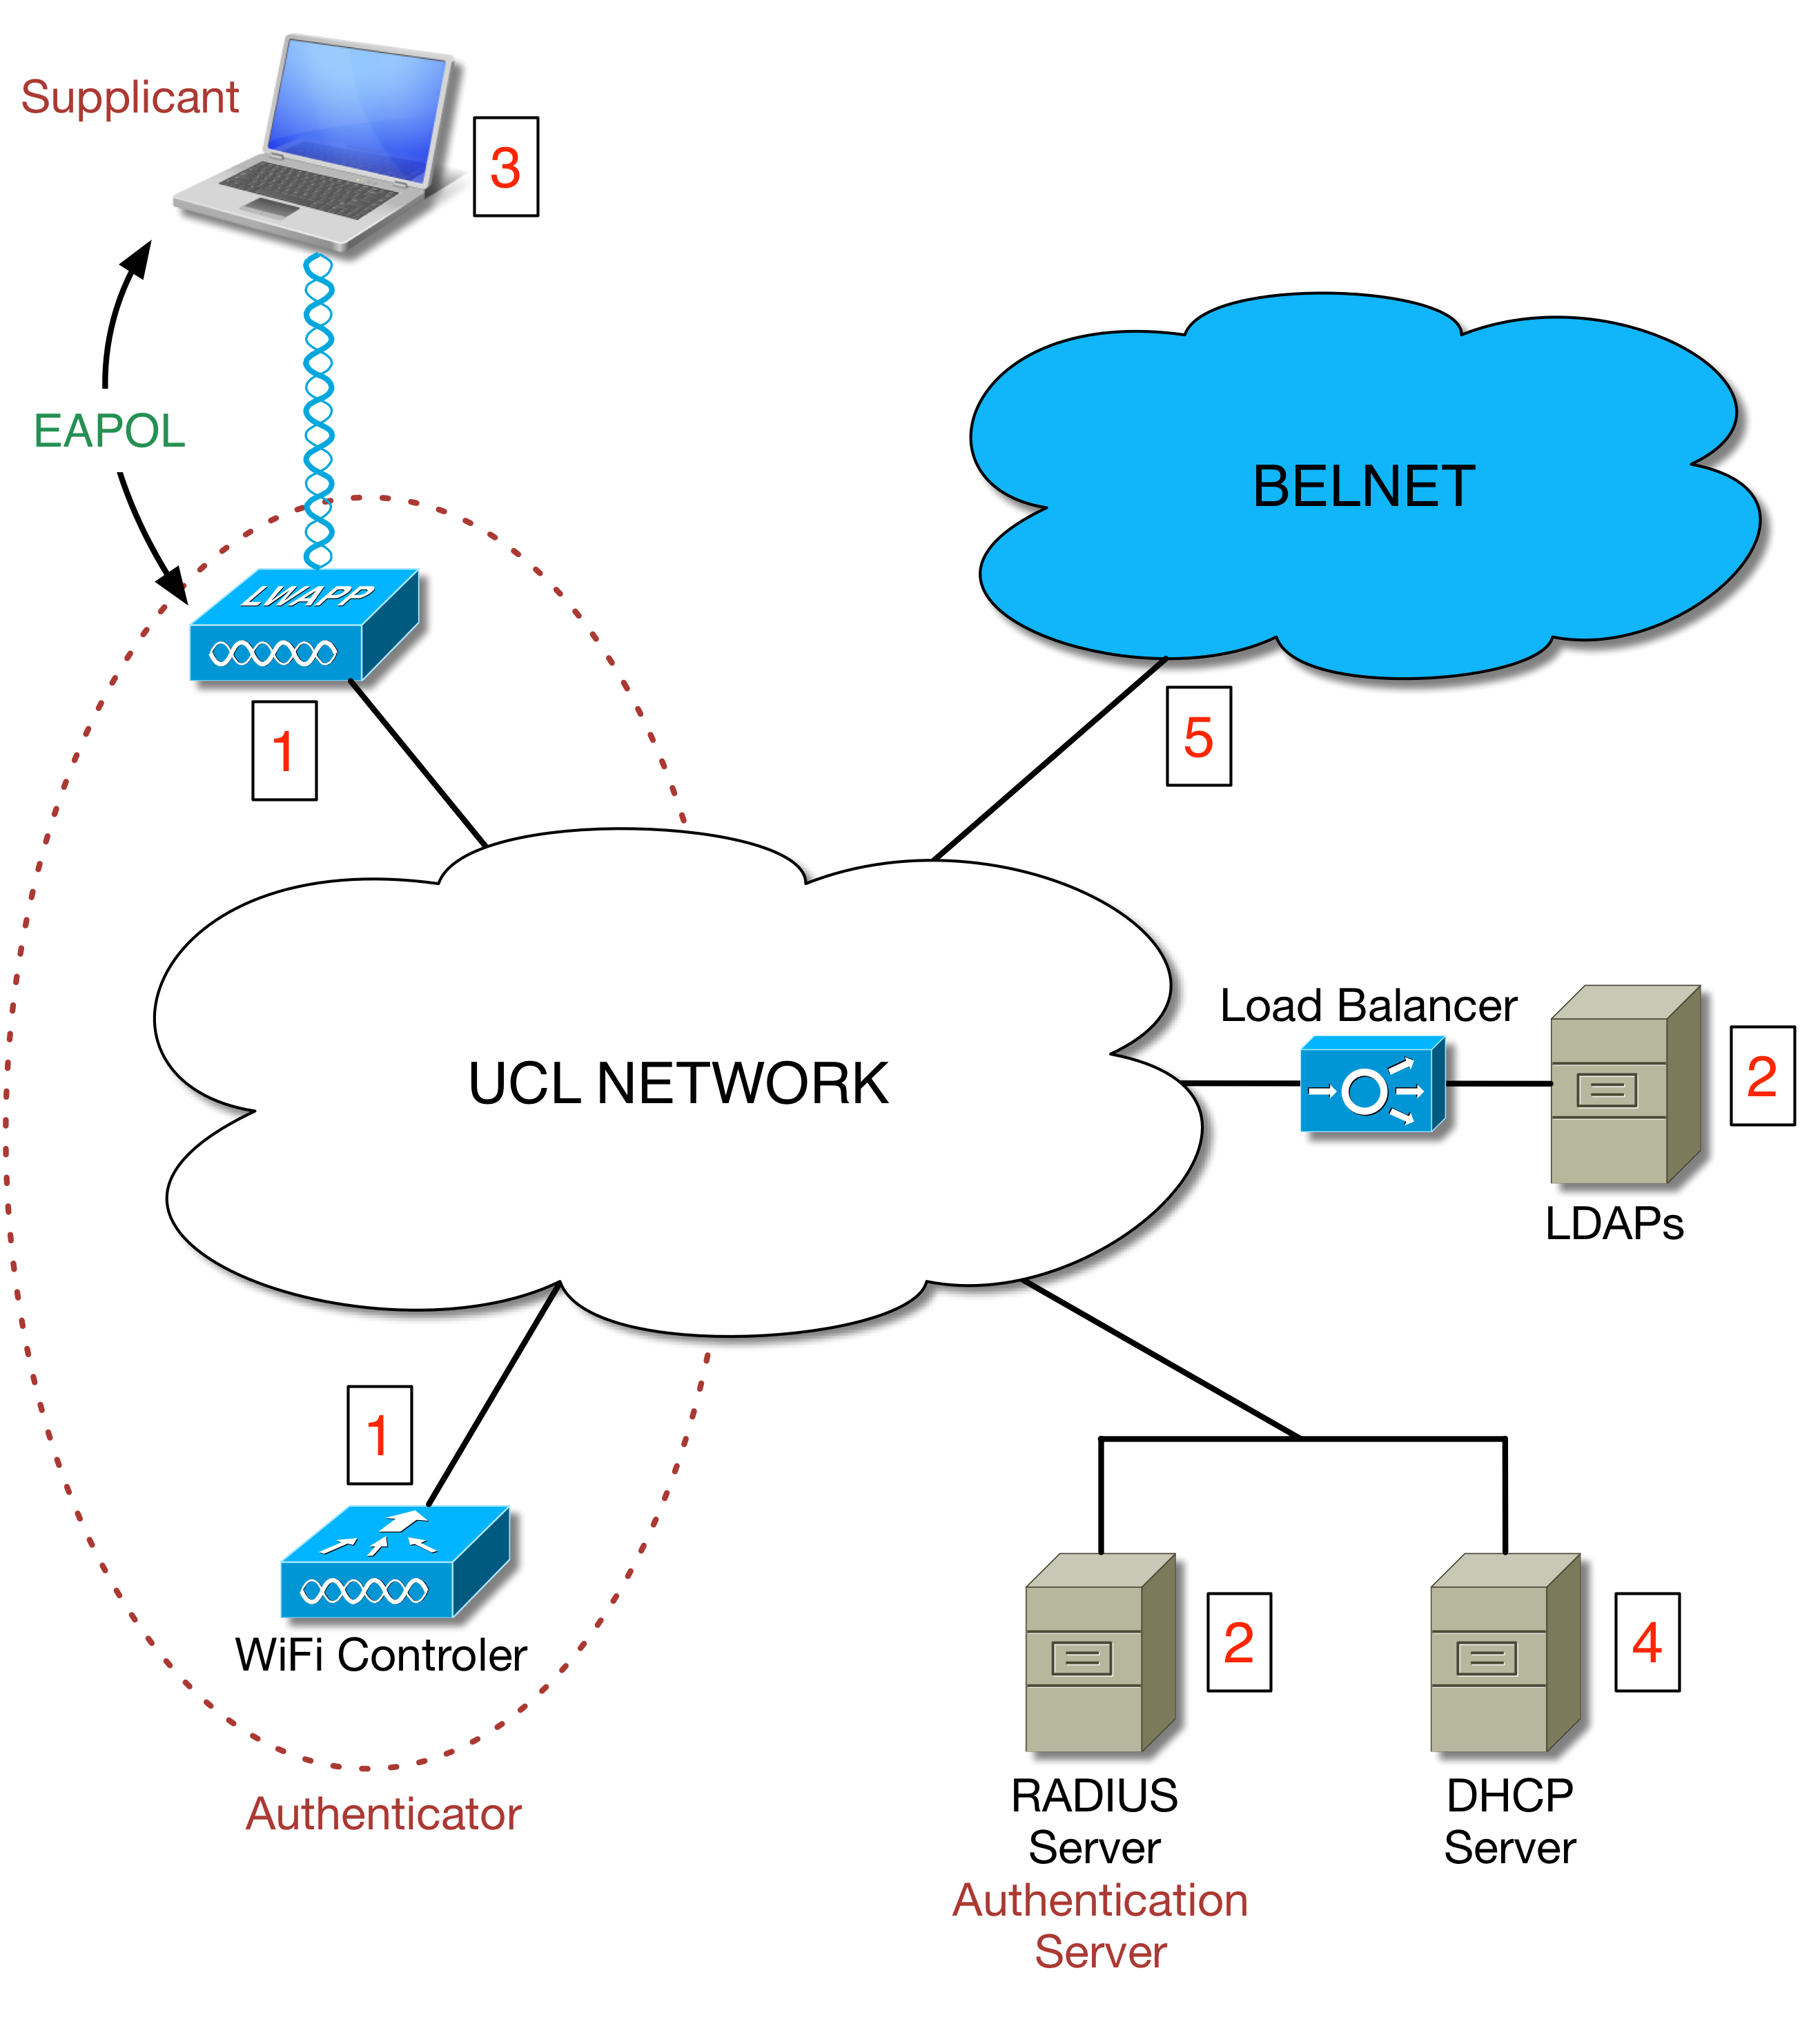
\includegraphics[width=.9\linewidth]{Pictures/chapter2/topology2.png}
	\caption{Authentication process on a UCL's WLANs}
\end{figure}


\subsection{student.UCLouvain authentication example}
To illustrate how the whole authentication process works, let's take a closer look to what happens when a student wants to connect to the \texttt{student.UCLouvain} network.
As detailed above, this network is protected by the \texttt{802.1X} authentication protocol. Thus the client first needs to authenticate himself before being able to access the Internet.
As a reminder, the client who wants to connect the network is called the \textit{supplicant}. This supplicant is going to first make a standard \texttt{802.11} association with the authenticator using \texttt{WPA/WPA2}. The authenticator is composed of the access point to which the supplicant is trying to connect and the WLAN controller that is going to handle the whole authentication request. Once this association has been made, the authenticator understands that the supplicant wants to get an access to the protected network and thus a \texttt{802.1X} session between them is started. At this state, only \texttt{802.1X} traffic is allowed (i.e. only \texttt{EAP} messages are accepted during the transmissions).

The first message the supplicant is going to send to the authenticator is an \texttt{EAPOL-Start} frame in order to initiate the authentication process. When the authenticator receives that frame, it sends an \texttt{EAP-Request Identity} frame to the supplicant that answers with an \texttt{EAP-Response Identity} frame containing the supplicant's identity. The authenticator encapsulates this response in a \texttt{RADIUS Access-Request} packet and forwards it to the authenticator server.

Once the authentication server has received that packet it sends a \texttt{RADIUS Access Challenge} back to the authenticator containing an \texttt{EAP Request} specifying the type of \texttt{EAP} method to use (\texttt{TTLS} or \texttt{PEAP}) in order to validate the identity of the supplicant and to specify how the credentials are submitted. The authentication server also sends its certificate during that negotiation. The authenticator encapsulates that \texttt{EAP Request} in an \texttt{EAPOL} frame and sends it to the supplicant.

Since the supplicant has a copy of the server certificate, it can checks if the one received during the negotiation is the same in order to authenticate the server's identity. Once its identity has been proved, the supplicant builds a \texttt{TLS-encrypted} tunnel with the authentication server. It then sends its credential securely inside this channel.

The authentication server validates the username and password of the supplicant and sends back a \texttt{RADIUS Access-Accept} packet to the authenticator that sends an \texttt{EAP-Success} frame to the supplicant. The authenticator opens the port for the supplicant and by doing so, completing the process of authentication and allowing the user to access the Internet after having negotiated a \texttt{WPA/WPA2} key with the authenticator in order to encrypt the further transmissions.

The following figure represents the main steps of the authentication process for the \texttt{student.UCLouvain} network:

\begin{figure}[H]
	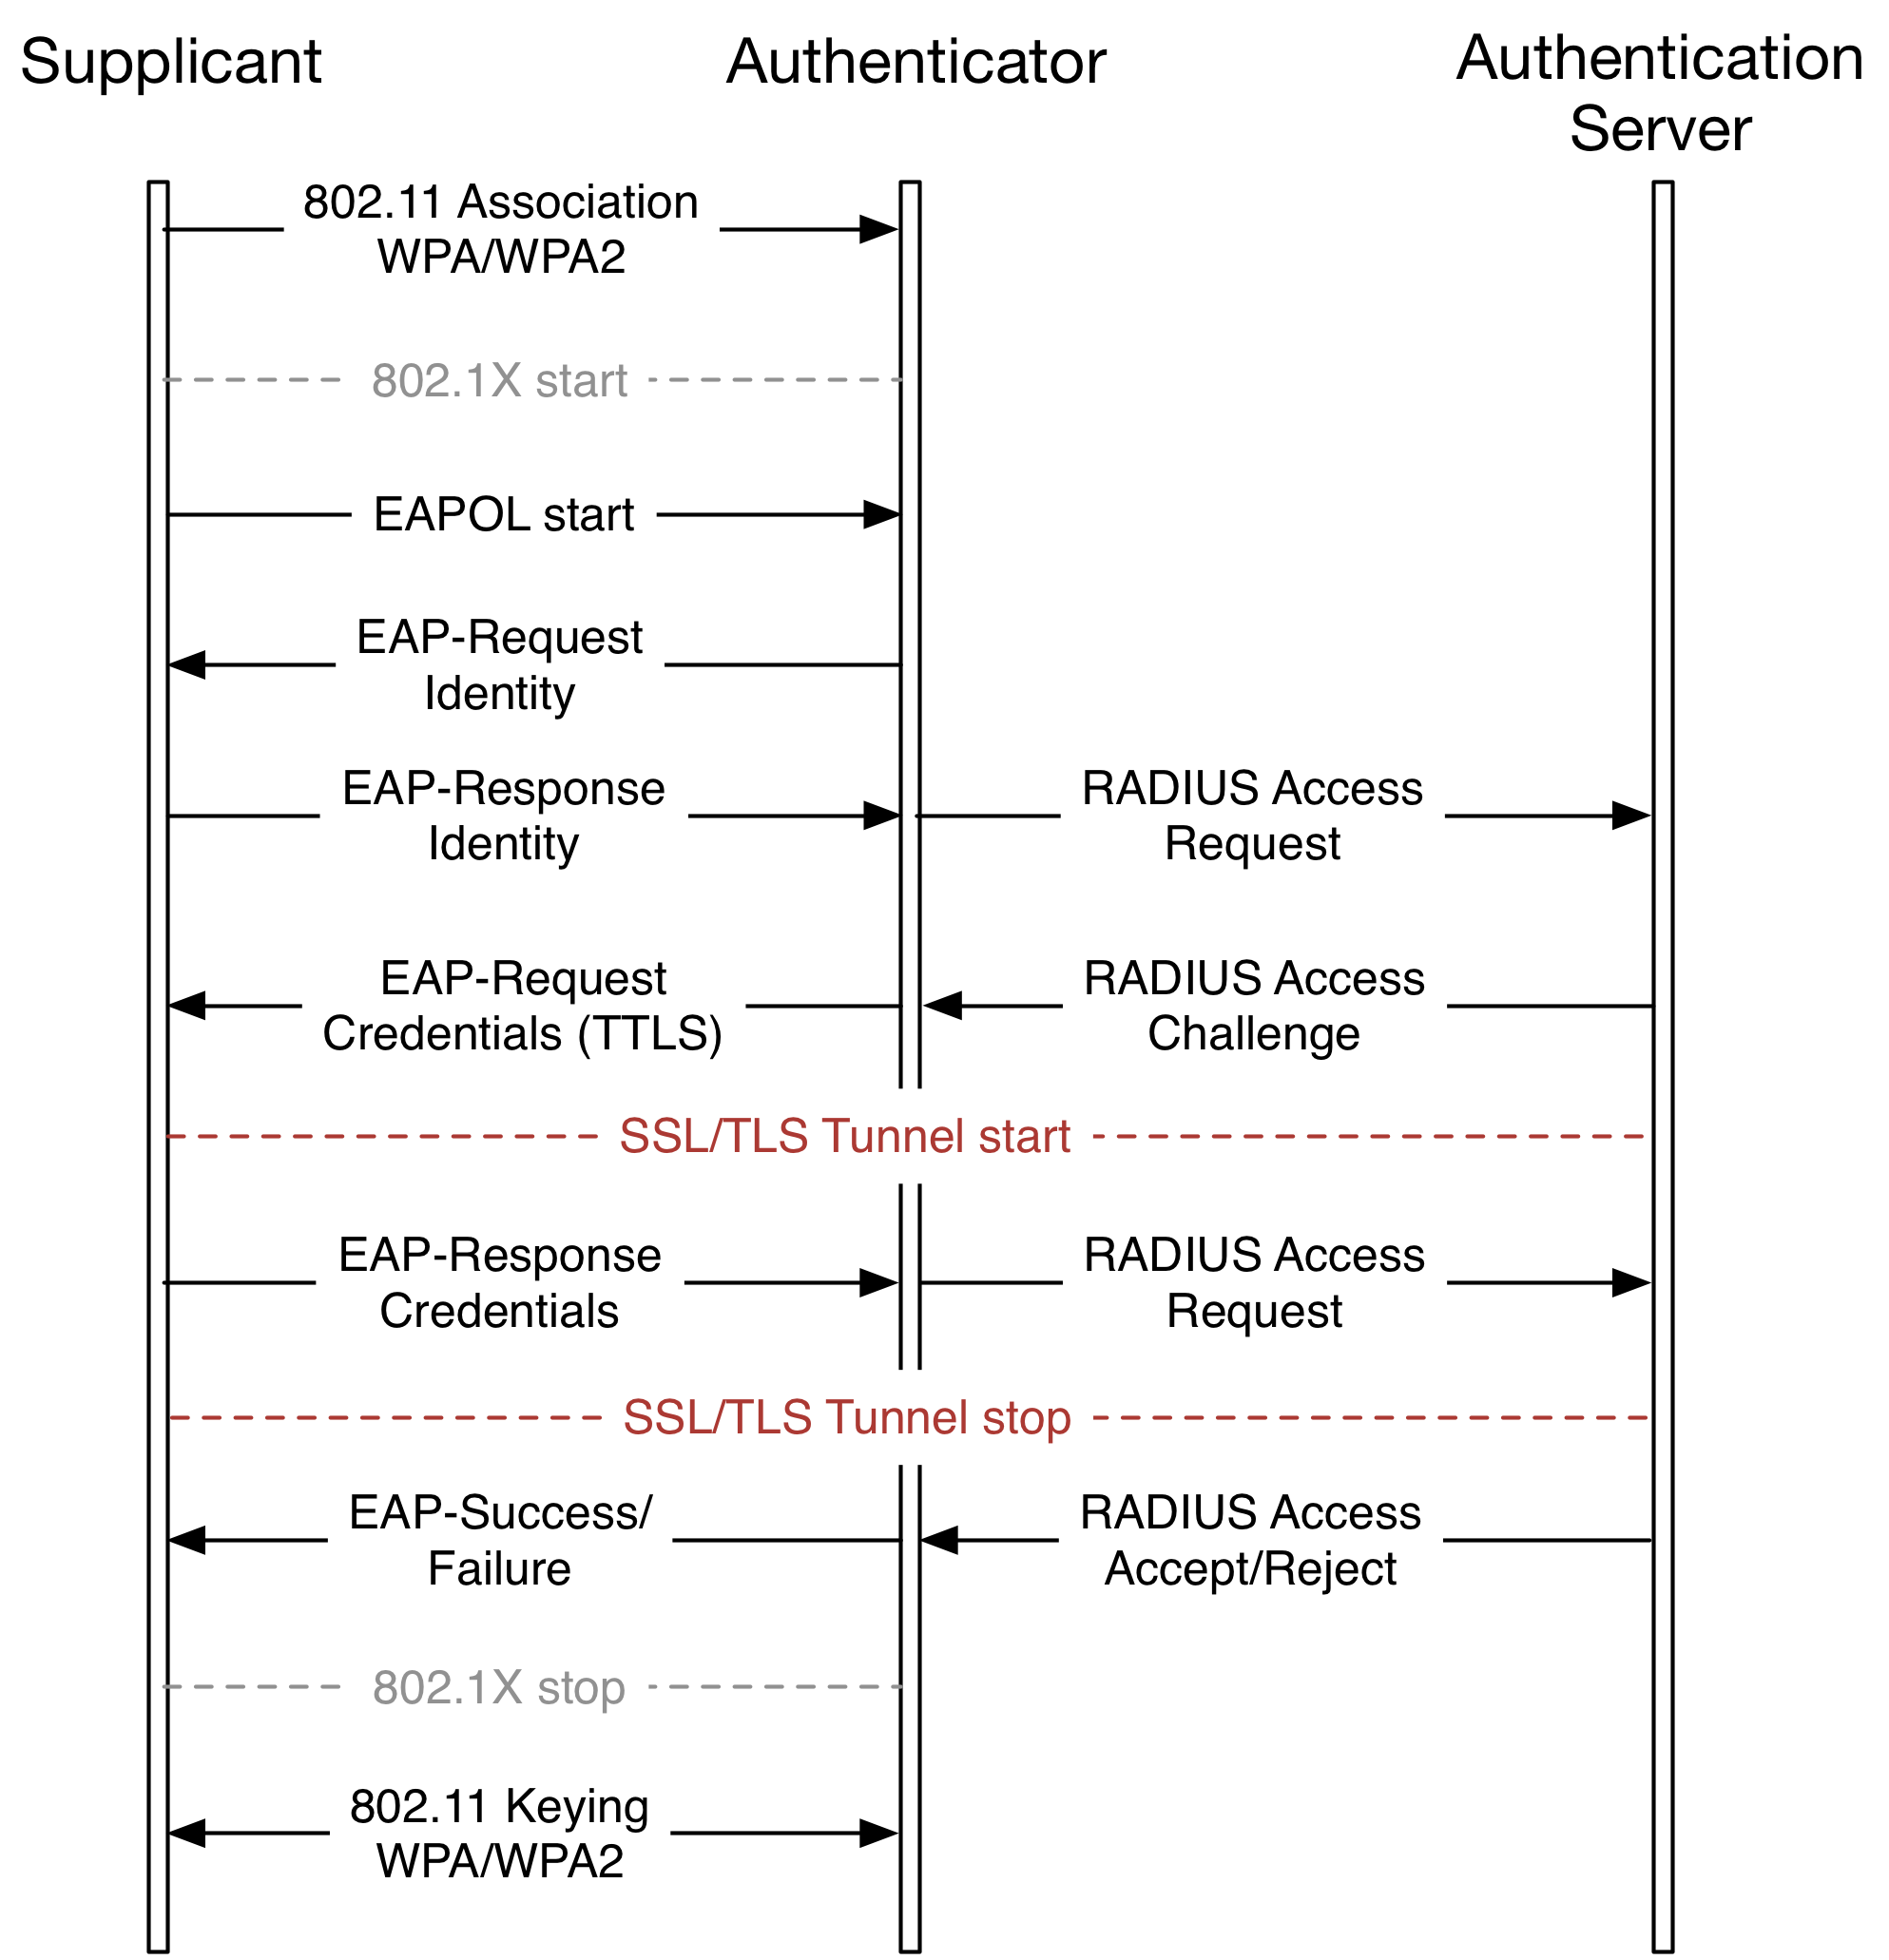
\includegraphics[width=.9\linewidth]{Pictures/chapter2/student.png}
	\caption{student.UCLouvain authentication process}
\end{figure}


\subsection{eduroam authentication example}
Let's take another WLAN authentication process example with the \texttt{eduroam} network which is a bit different than the example seen before.
As explained in \cite{eduroamRadius}, the \texttt{eduroam} project is "\textit{A wolrdwide federation of} \texttt{RADIUS} \textit{ servers facilitating network access for roaming academic affiliates using} \texttt{IEEE 802.1X} \textit{as the vehicle. eduroam's use of} \texttt{802.1X} \textit{in concert with} \texttt{RADIUS} \textit{means the network is built around well understood, established, and easy to manage standards which are often already deployed within the network infrastructure of educational institutions}".

Since \texttt{eduroam} is also using the \texttt{802.1X}, when a client wants to connect to the network, he is not able to pass any traffic other than \texttt{802.1X} until his request is accepted by the authentication server. As for the \texttt{student.UCLouvain} network, the communication between the supplicant and the authenticator also involves \texttt{EAP} conversation.The supplicant sends its \texttt{EAP} messages to the authenticator that forwards them to the authentication server in the form of a \texttt{RADIUS} request. To ensure the protection of the credentials and information sent during the authentication negotiation, eduroam uses either \texttt{TTLS} or \texttt{PEAP} (\textit{Protected Extensible Authentication Protocol}).A \texttt{TLS-encrypted} tunnel is also created between the supplicant and the authentication server.

As a student from another university than the Catholic University of Louvain can access and connect to the \texttt{eduroam} network from inside the Louvain-la-Neuve campus, the local authentication server, in Louvain-la-Neuve, is not the one that is going to handle the authentication request. Indeed, if the user comes from the University of Seville in Spain, for example, its authentication request within the UCL's campus is first handled by the local \texttt{RADIUS} server. This server forwards the request to the Belnet \texttt{RADIUS} server since it does not know the realm used by the Spanish student. That Belnet server understands that this student is not from Belgium. It thus forwards the request to the European \texttt{RADIUS} server, Terena. Terena understands that the user comes from Spain so it forwards the request to the Spanish national \texttt{RADIUS} server that finally forwards the request to the University of Seville's server. The response takes the same route to get to Louvain-la-Neuve.

The \texttt{RADIUS} protocol supports that forwarding in its proxy mode. To prevent any administrators not responsible for the handling of the authentication request, the \texttt{TLS-encrypted} tunnel is propagated throughout the \texttt{RADIUS} infrastructure. Thanks to that tunnel, the intermediate authenticator does not handle sensitive information during the authentication process.

Here is a representation of the authentication request communications between the supplicant, the authenticator and the authentication server with \texttt{RADIUS} proxying:
\begin{figure}[H]
	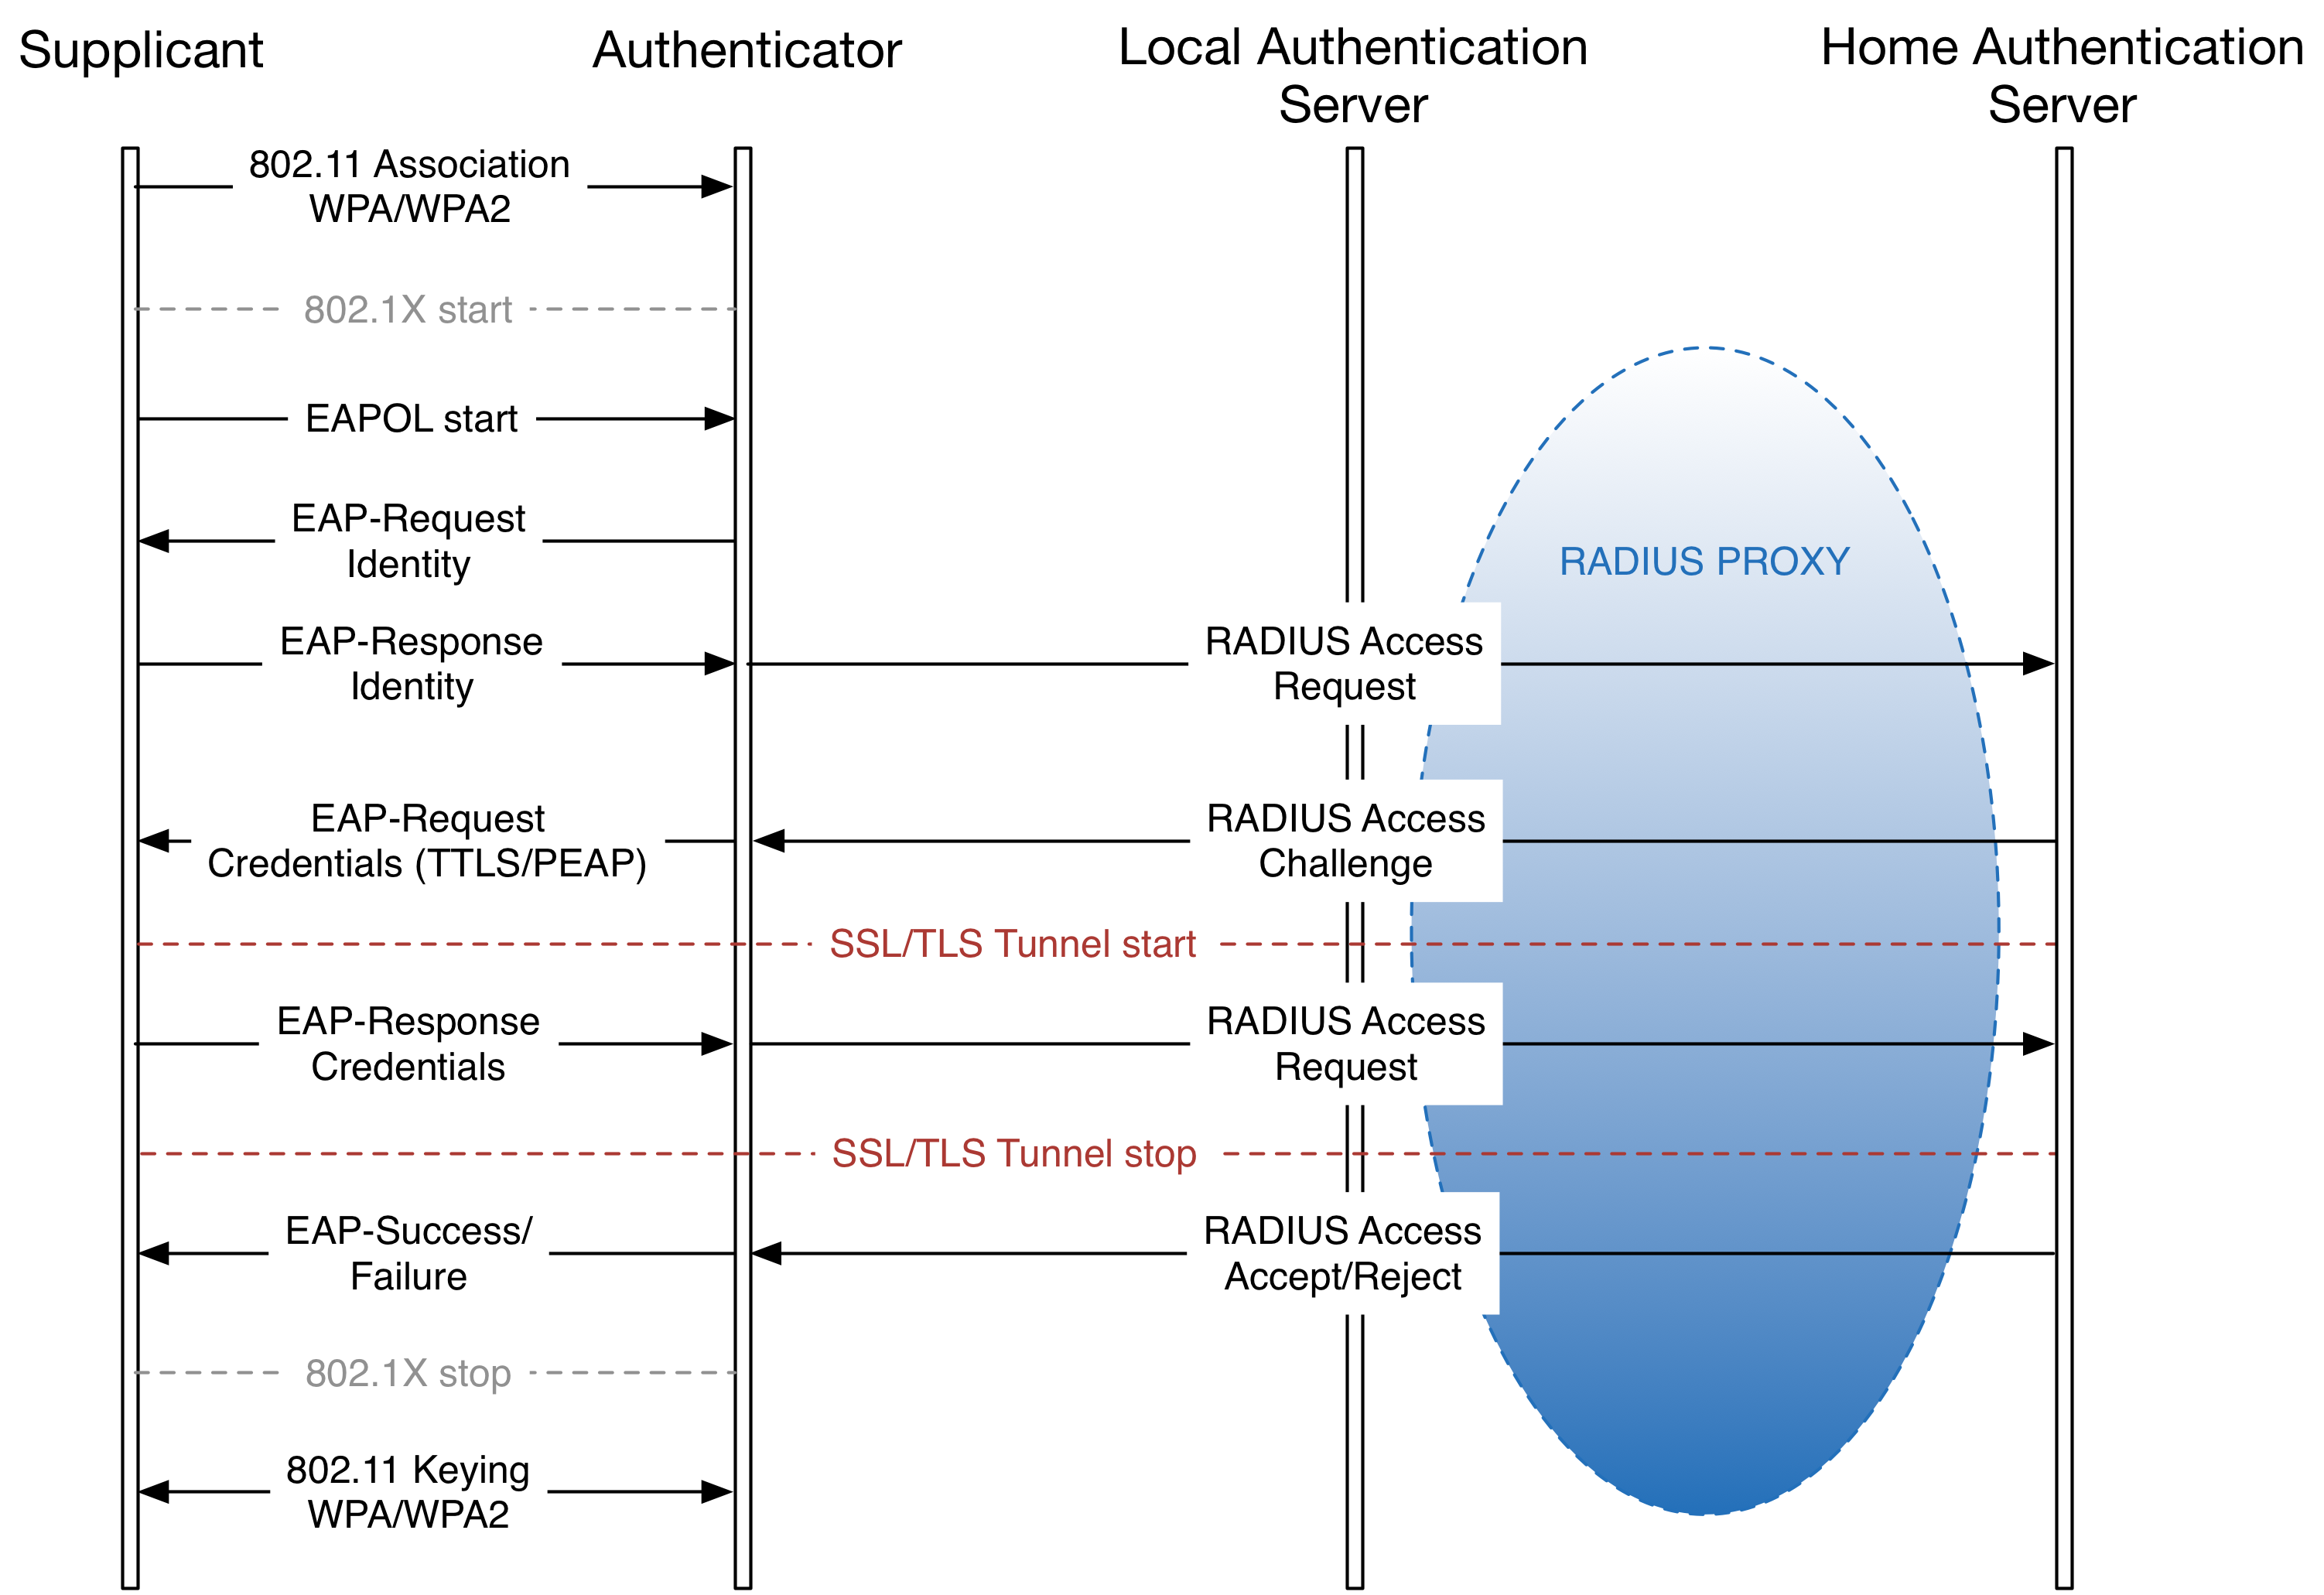
\includegraphics[width=1\linewidth]{Pictures/chapter2/eduroam1.png}
	\caption{eduroam authentication process}
\end{figure}

\section{Infrastructure architecture}
Within the Catholic University of Louvain's network infrastructure architecture, the Internet access is provided by Belnet via a 10Gbit Ethernet link. This link is connected to one of the seven \textit{neighborhood routers} called \texttt{CtPythagore}. There is also a second 1Gbit Ethernet link connected to another neighborhood router called \texttt{CtHalles}. This second link is never used and is, in fact, a backup link in case of a failure of the main one.

The other neighborhood routers are \texttt{CtLew}, \texttt{CtStevin}, \texttt{CtCarnoy}, \texttt{CtMichotte} and \texttt{CtSHI1C}. They are all on the Louvain-la-Neuve campus expect for \texttt{CtLew} that lies on the Woluwe campus in Brussels. Those neighborhood routers are all \texttt{Cisco Catalyst 6509} switches and are the campus core routers. Two of them (\texttt{CtSH1C} and \texttt{CtMichotte}) include a \texttt{Cisco WiSM2} (\textit{Wireless Services Module 2}) controller. The infrastructure also contains two data centers called \texttt{CtTier2} and \texttt{CtAquarium}. Each one of those data center has a load balancer. The two \texttt{DHCP} servers as well as the \texttt{LDAP} servers are located behind those load balancers.

Here is a representation of the UCL's network infrastructure.

\begin{figure}[H]
	
\includegraphics[width=1\linewidth]{Pictures/chapter2/ucl.png}
	\caption{UCL's network infrastructure architecture}
\end{figure}


Each building on the Louvain-la-Neuve campus has a direct connectivity with the network. Inside there are several access points (there are approximatively 300 access points on the Louvain-la-Neuve's campus and most of them are \texttt{Cisco AIR-AP1242AG}. Yet they are starting to be replaced, only in the INGI buildings for this moment, by either \texttt{Cisco Aironet 3600} or \texttt{Cisco Aironet 3700}) that provide an Internet access to the clients. Each access point is connected to a switch \texttt{Cisco Catalyst 2960-48LPS}. This switch only has 48 ports so there are several one of them, in each building, place in a patch room. Those switches are connected to another switch \texttt{Cisco Catalyst 2960G-24TC-L} that has a direct fiber connection with one of the seven neighborhood routers. Thanks to that connection, each building is connected to the UCL network and thus, to the WiFi controller.

The following figure represents a simplified overview of how the buildings are connected to the network.

\begin{figure}[H]
	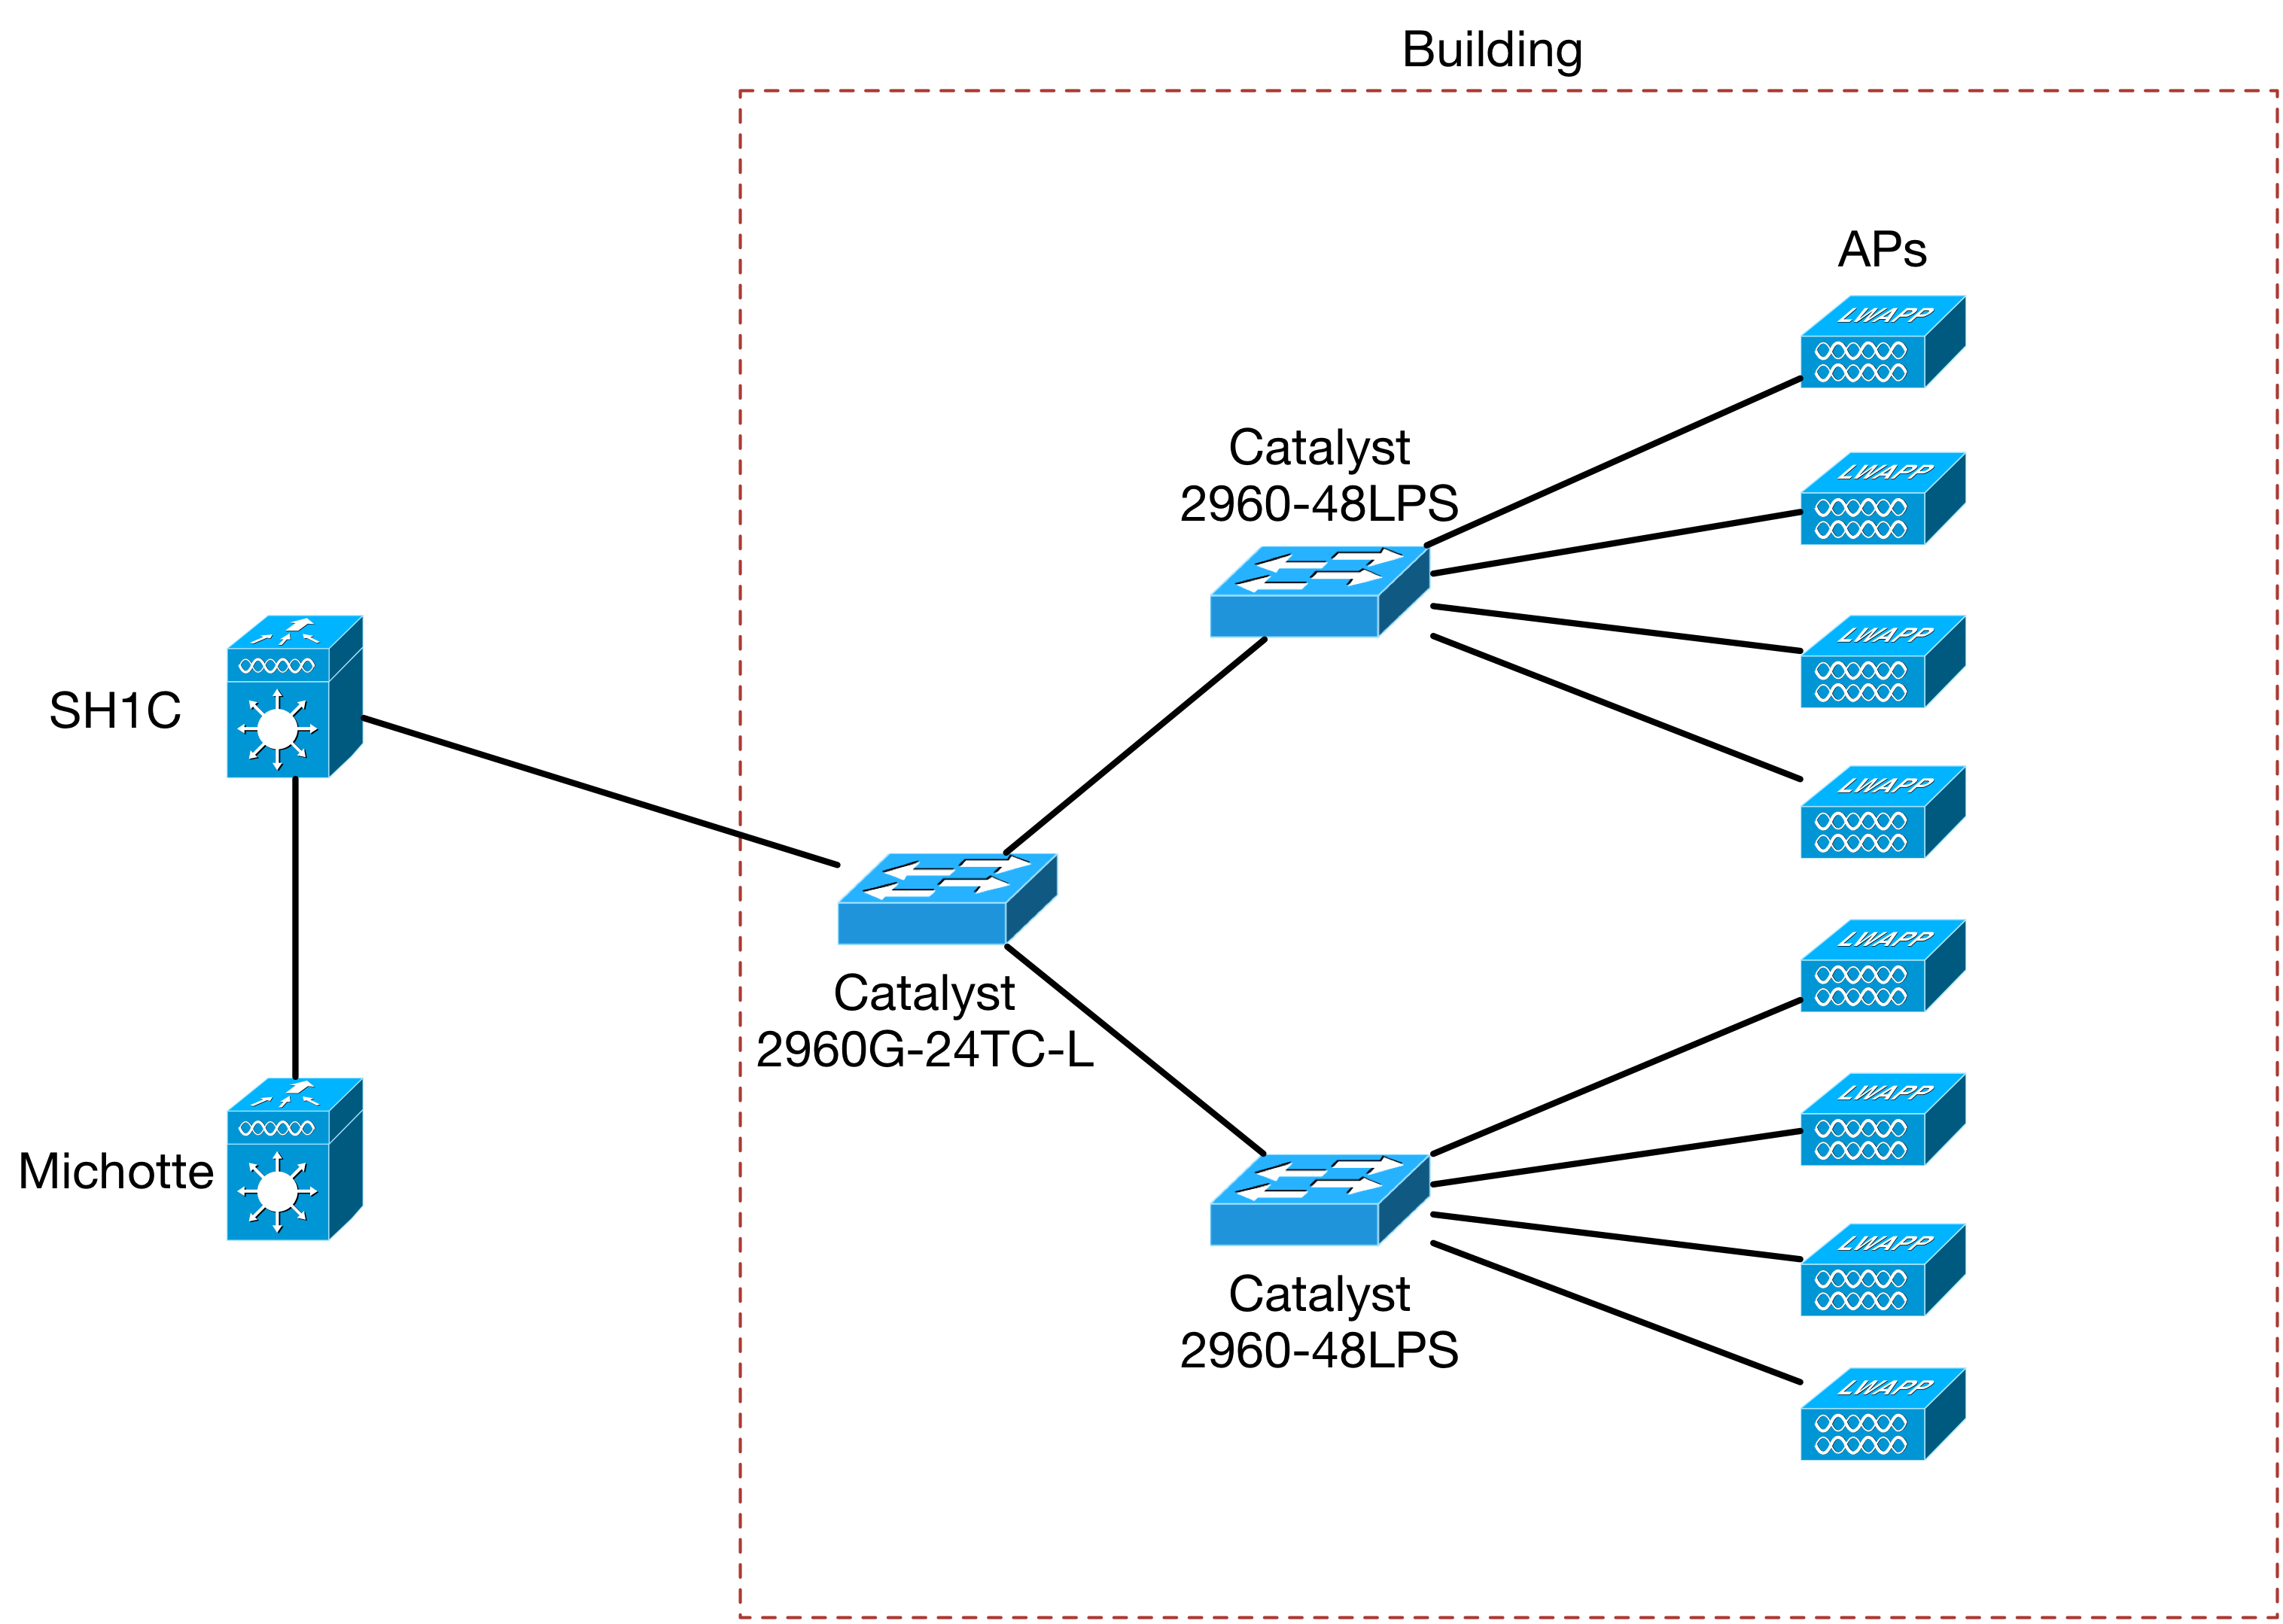
\includegraphics[width=1\linewidth]{Pictures/chapter2/building.png}
	\caption{Building infrastructure and network connection}
\end{figure}


\section{Summary}
This chapter reviewed the relevant components and protocols used inside the Catholic University of Louvain's wireless infrastructure. \texttt{WLAN} authentication process as well as the entire infrastructure's architecture were also developed and detailed. With this background, we can now move on to the monitoring tool architecture, implementation and deployment. Later chapters discuss analysis and results made in the deployment phase.





